\documentclass[10pt,a4paper]{article}
%\usepackage[utf8]{inputenc}
\usepackage[T1]{fontenc}
\usepackage{amsmath}
\usepackage{amsfonts}
\usepackage{amssymb}
\usepackage{graphicx}
\usepackage{float}
\usepackage{tikz-cd}
\usepackage{mathtools}
\usepackage{enumitem}
%\renewcommand{\figurename}{Rysunek}

\usepackage{algorithm,algorithmic}

\usepackage{polski}
\usepackage[polish]{babel}
%\usepackage{fontspec}
%\usepackage[nosingleletter]{impnattypo}
\usepackage{hyper/ref}
\hypersetup{
	colorlinks=true,
	linkcolor=blue,
	filecolor=magenta,      
	urlcolor=cyan,
}
% dr ratajczak
% ziomek

\author{Wojciech Sopot 235291}
\title{Filtry cząsteczkowe i ich zastosowanie w lokalizacji}
\begin{document}
\maketitle
\tableofcontents
\newpage
\section{Wprowadzenie}W rozdziale przedstawiono podstawowe zadania i problemy wyznaczania lokalizacji oraz ogólną ideę stojącą za filtrami cząsteczkowymi - filtrację bayesowską.
\subsection{Zadania i problemy wyznaczania lokalizacji}
Mogłoby się wydawać, iż w dzisiejszych, gdy mamy możliwość korzystania z systemu GPS, nie ma potrzeby zajmować się innymi sposobami wyznaczania lokalizacji. Jednak o ile jest to prawdą w dużej skali, jak np. gdy chce się wyznaczyć adres w mieście pod którym się znajdujemy, to gdy chcemy wyznaczyć swoją lokalizację bardziej dokładnie, np. jak to robią niektóre odkurzacze mobilne, to trzeba wykorzystać do tego dane z innych sensorów, np. lidarów. Czasami można wcale nie mieć możliwości korzystania z systemu GPS, na przykład pod wodą. Innym problemem może być poprawa już znanego przybliżonego położenia. W pracy zostaną przeanalizowane dwa problemy związane z wyznaczaniem lokalizacji:
\begin{itemize}
	\item Określanie położenia samolotu, na podstawie znanej mapy wysokościowej terenu, odczytów z wysokościomierza barometrycznego, oraz, ewentualnie, dodatkowych danych (np. odczytu z kompasu). Warto zauważyć, iż jest to problem analogiczny do łodzi podwodnej orientującej się na podstawie odległości od dna.
	\item Określanie lokalizacji robota mobilnego, umieszczonego w ograniczonej przestrzeni z przeszkodami (ale na płaskiej powierzchni - mapa jest w dwóch wymiarach).
\end{itemize}
\subsection{Cel pracy}
\subsection{Zakres pracy}
\subsection{Filtracja Bayesowska}
Na chwilę obecną, algorytmy oparte o filtrację Bayesowską są szeroko wykorzystywane w automatyce i robotyce. W skrócie, podejście to polega na przeprowadzaniu cykli predykcji i poprawek na podstawie znanego a priori stanu, oraz zbieranych w kolejnych iteracjach pomiarów. Ideę tego podejścia widać na rysunku \ref{bayes_fil_idea}. 
\begin{figure}[H]
	\begin{center}
		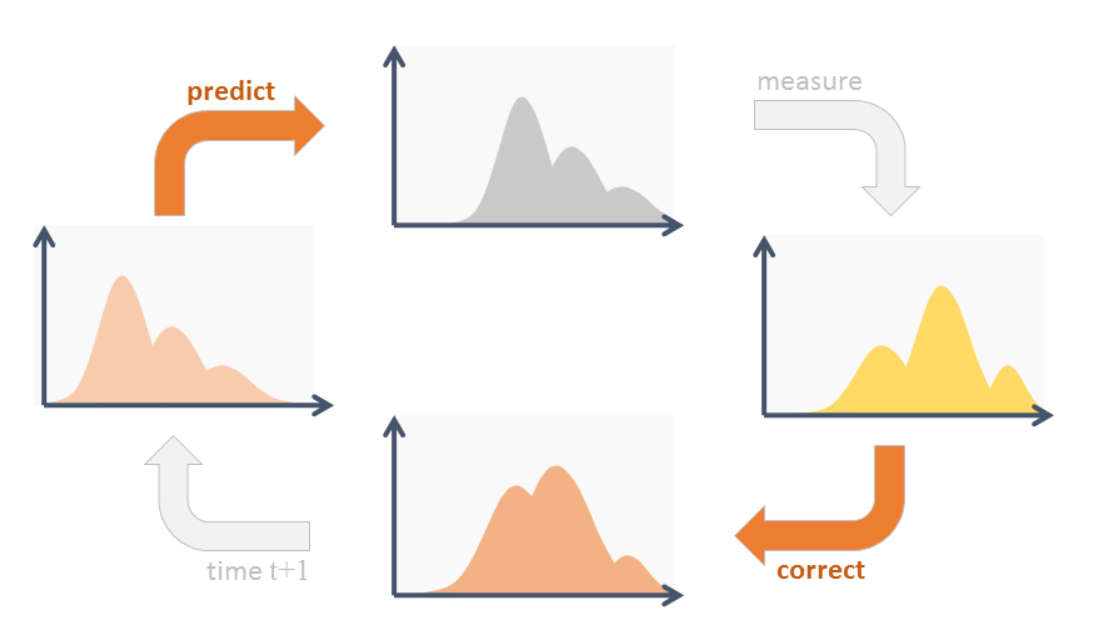
\includegraphics[width=10cm]{./predict_update.png}
		\caption{Idea filtracji Bayesowskiej. Obrazek zaczerpnięto z https://www.codeproject.com/Articles/865934/Object-Tracking-Particle-Filter-with-Ease}
		\label{bayes_fil_idea}
	\end{center}
\end{figure}
Na rysunku \ref{filtr_hier} przedstawiono hierarchię rozwiązać opartych o to podejście. W pracy zostaną poruszone metody oparte o filtry cząsteczkowe.
\begin{figure}
	\begin{center}
		\includegraphics[width=10cm]{./nfg001.jpg}
		\caption{Hierarchia filtrów opartych o filtrację Bayesowską. Obrazek zaczerpnięto z \cite{prac_gui}}
		\label{filtr_hier}
	\end{center}
\end{figure}
\section{Filtry cząsteczkowe}
%\subsection{Pojęcia podstawowe}
\subsection{Opis problemu}
Celem filtru cząsteczkowego jest wyznaczenie rozkładu zmiennej stanu $X_k$, na podstawie szczątkowych pomiarów $Y_k$ za pomocą filtracji Bayesowskiej. \\
\begin{equation*}
\begin{tikzcd}
	X_0 \arrow{r} \arrow{d} &X_1 \arrow{r} \arrow{d} &X_2 \arrow{r} \arrow{d} &X_3\arrow{r} \arrow{d} &...\\
	Y_0 &Y_1 &Y_2 &Y_3 &...
\end{tikzcd} 
\end{equation*}
System taki, można opisać w następujący sposób
\begin{equation*}
	\begin{aligned}
		X_k=g(X_{k-1})+W_{k-1} \\
		Y_k=h(X_k)+V_k
	\end{aligned}
\end{equation*}
TODO małą gdzie $g$ i $h$ to znane funkcje, a $W_{k-1}$ i $V_k$ to szumy. Jeśli oba szumy byłyby z rozkładu normalnego, a $g$ i $h$ są liniowe, to problem można rozwiązać za pomocą filtru Kalmana. Aby zyskać na ogólności, System można opisać w następujący sposób:
\begin{equation}
	\begin{aligned}
		X_k=g(X_{k-1}, W_{k-1}) \\
		Y_k=h(X_k, V_k)
	\end{aligned}
\end{equation}

\subsection{MAtematyczny opis filtracji Bayesowska}
Ogólne wzory na filtrowanie Bayesowskie:
\begin{equation}
	p(X_k|Y_{0...k})=\frac{p(Y_k|X_k)p(X_k)}{p(Y_k|Y_{0...k-1})}
\end{equation}
\begin{equation}
p(Y_k|Y_{0...k})=\int p(Y_k|X_k)p(X_k|Y_{0...k-1}) dX_k
\end{equation}
\begin{equation}
p(X_k|Y_{0...k-1})=\int p(X_k|X_{k-1})p(X_{k-1}|Y_{0...k-1}) dX_{k-1}
\end{equation}
TODO cytat
Można zauważyć, iż wzór (3) jest stały względem $X_k$, jest to, tak zwana stała normalizacyjna. Wiedząc to, i podstawiając wzory (3) i (4) do (2) uzyskujemy:
\begin{equation}
	p(X_k|Y_{0...k})=\mu p(Y_k|X_k)\int p(X_k|X_{k-1})p(X_{t-1}|Y_{0...t-1}) dX_{t-1}
\end{equation}
Gdzie $\mu$ jest stałą normalizacyjną.
\subsection{Importance sampling i regularyzacja}
Równanie (5) stanowi podstawę konstrukcji wielu algorytmów....\\
Istotna trudność w jego zastosowaniu polega jednak na tym, 

Aby móc w praktyce zrealizować równanie (5), trzeba skorzystać z dwóch konceptów - importance samplingu(IS) i regularyzacji. \\
Nie wiem czy jest sens to opisywać, bo koniec końców to się sprowadza do opisu algorytmu w kolejnym rozdziale
\subsection{Podstawowy algorytm filtra cząsteczkowego}
W filtrze cząsteczkowym, ciągłe rozkłady $p(\bullet)$ są symulowane za pomocą chmury ważonych cząstek. Każda cząstka wygląda w następujący sposób:
\begin{equation*}
	p_i=\{x_{k,i},w_{k,i}\}
\end{equation*}
Gdzie $x_{k,i}$ to stan w iteracji $k$ związany z cząstką $i$, $w_{k,i}$ to jej waga.
Początkowo całą populację cząstek inicjuje się cząstkami z losowymi stanami i wagami, równymi dla każdej cząstki. Następnie wykonuje się w pętli:
\begin{enumerate}[label=(\alph*)]
	\item Wyznacza się nowy zbiór cząstek, dla każdej cząstki $x_{k,i}$ uzyskuje się, symulując jej ewolucję, w oparciu o $x_{k-1,i}$. Model ruchu powinien uwzględniać szumy obecne w systemie.
	\item Pojawia się nowy pomiar $Y_k$, na podstawie którego na którego podstawie modyfikuje się wagi poszczególnych cząstek.
	\item Wagi są normalizowane.
	\item Wyznacza się estymowany stan, wyznaczając ważoną średnią stanów wszystkich cząstek.
	\item Wyznacza się efektywną liczbę cząstek według wzoru:
	\begin{equation*}
		N_{eff_k} = \dfrac{1}{\sum w_{k,i}^2}
	\end{equation*}
	Jeśli jej wartość jest mniejsza, niż pewien próg, to przeprowadza się ponowne próbkowanie, generując nową populację cząstek (jest to sztuczka pozwalająca na ograniczenie liczby obliczeń, teoretycznie próbkowanie można przeprowadzać co iterację).
\end{enumerate}


\subsection{Adaptacyjna liczba cząstek}
Oczywistym jest, że największy wpływ na złożoność obliczeniową filtra cząsteczkowego ma ilość cząstek. W \cite{adaptive} opisano algorytm który służy do dynamicznego zmieniania liczby cząstek. Polega on na zmodyfikowaniu kroku (e) podstawowego algorytmu, gdzie tuż przed próbkowaniem wyznacza się nową liczbę cząstek, korzystając z poniższego algorytmu.

\begin{figure}[H]
	\begin{center}
		\includegraphics[width=10cm]{./adaptive_algo.png}
		\caption{Algorytm adaptacyjnego doboru liczby cząstek. Obrazek zaczerpnięto z\cite{adaptive} - TODO DODAĆ (8):y-h}
		%\label{bayes_fil_idea}
	\end{center}
\end{figure}

W skrócie, algorytm polega na sprawdzaniu, które cząstki leżą zbyt blisko siebie, a następnie ich stopniowemu usuwaniu, badając jak to wpływa na jakość jakość estymacji. Na koniec o nową liczbę cząstek określa się tak, aby pogorszenie estymacji nie było większe niż pewien próg.

\subsection{Box Particle Filter}
W tym podejściu zaproponowanym w \cite{bpfln}TODO i udoskonalonym w \cite{brbpf} zmieniono sposób reprezentacji cząstek, ponieważ zamiast punktów w przestrzeni stanów zastosowano interwały. Może się wydawać, iż zwiększy to złożoność obliczeniową, ponieważ trzeba o wiele więcej czasu poświęcić na analizę poszczególnych cząstek, jednak dzięki temu możemy zredukować samą ich liczbę.

\begin{figure}[H]
	\begin{center}
		\includegraphics[width=10cm]{./bpf_algo.png}
		\caption{Algorytm Box Particle Filter}
		%\label{bayes_fil_idea}
	\end{center}
\end{figure}

Powyższy algorytm nie posiada wszystkich usprawnień zaproponowanych w \cite{brbpf}. Wykorzystano jedynie reinicjalizację, gdy wszystkie wagi się wyzerują.

\subsection{Wprowadzenie operatora mutacji}
W \cite{pfgen} zaproponowano, aby wzbogacić proces próbkowania o operatory krzyżowania i mutacji.

\begin{figure}[H]
	\begin{center}
		\includegraphics[width=10cm]{./genetic_pf.png}
		\caption{Genetyczny filtr cząsteczkowy. Obrazek zaczerpnięto z \cite{pfgen}.}
		%\label{bayes_fil_idea}
	\end{center}
\end{figure}

%\subsection{Najczęstsze zastosowania}
%\cite{appl3} \cite{applg}
%\subsection{Przegląd aktualnych usprawnień} \label{przeg}
%\section{Filtry cząsteczkowe} \label{przeg}
\section{Wybrane narzędzia programistyczne}
\section{Badania} \label{przeg}
Będę badać wpływ kolejnych usprawnień znalezionych w literaturze, obrazki + tabelki.
\subsection{Badania poprawności działania}
\subsubsection{Wpływ generatora}
mam nadzieję, że będzie tak samo XD
\subsubsection{Brak pkt odniesienia}
wiele równoważnych położeń
\subsubsection{Brak ewolucji systemu}
Powinny się pojawić izolinie.

\subsection{Wpływ sposobu estymowania położenia}
\subsection{Wpływ sposobu estymowania położenia}
\subsection{Wpływ liczby cząstek}
\subsection{Wpływ metody próbkowania}
\subsection{Skuteczność w poprawianiu błędnie określonego położenia}
\subsection{Wpływ szumu}
\subsection{Wpływ różnorodności terenu}

\section{Wnioski}
\begin{itemize}
	\item 
\end{itemize}
\section{Podsumawanie}
co w kolejnych rozdziałach

\subsection{Kierunki przyszłych badań}
\begin{itemize}
	\item Zrezygnowanie z implementacji C++ na rzecz całkowitego przejścia na Python, z wykorzystaniem na przykład pakietu Numba \cite{numba}. Poza przyspieszeniem porównywalnym z C++, pozwoliło by na przykład na poszerzanie kodu o obliczenia na karcie graficznej. Dzięki temu, można by spróbować rozwiązać problem robota w pokoju, wykorzystując Box Particle Filter.
	\item zamiast avg, np klasteryzacja?
\end{itemize}

\bibliographystyle{unsrt}
\bibliography{biblio}

\end{document}